% !TEX program=lualatex
\RequirePackage{luatex85}
\documentclass[10pt,tikz]{standalone}

\usepackage{luatextra} % also loads fixltx2e, fontspec, xunicode
\usepackage{microtype} % Slightly tweak font spacing for aesthetics
\usepackage{mathtools}
\usepackage{amsmath}
\usepackage{unicode-math}
\usepackage{xcolor}

\usepackage{tikz}
\tikzset{
  font={\fontsize{9pt}{11}\selectfont}
}

\usetikzlibrary{shapes,arrows,positioning}

\setmainfont{TeX Gyre Heros}
\setmathfont{Latin Modern Math}
\definecolor{colorR}{RGB}{228,26,28}    % RED
\definecolor{colorB}{RGB}{55,126,184}   % BLUE
\definecolor{colorG}{RGB}{77,175,74}    % GREEN
\definecolor{colorP}{RGB}{152,78,163}   % PURPLE
\definecolor{colorO}{RGB}{255,127,0}    % ORANGE
\definecolor{colorY}{RGB}{255,255,51}   % YELLOW
\definecolor{colorBn}{RGB}{166,86,40}   % BROWN
\definecolor{colorPk}{RGB}{247,129,191} % PINK
\definecolor{colorGy}{RGB}{153,153,153} % GRAY

\tikzstyle{line}=[draw, -stealth', very thick]
\tikzstyle{block}=[circle,fill=colorB!50,on grid]
\tikzstyle{lab}=[]
\tikzstyle{w}=[lab,midway]
\tikzstyle{e}=[lab,midway,auto=false,fill=colorP!50,font=\scriptsize]

\begin{document}
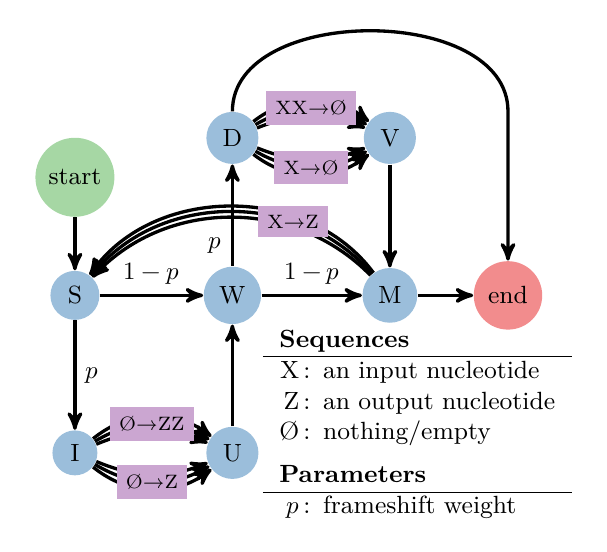
\begin{tikzpicture}[node distance=20mm, auto]
\clip (-6mm,19mm) rectangle +(70mm,-63mm);

\node[block,fill=colorG!50] (start) {start};
\node[block,below=15mm of start] (S) {S};
\node[block,right=of S] (W) {W};
\node[block,below=of S] (I) {I};
\node[block,right=of I] (U) {U};
\node[block,above=of W] (D) {D};
\node[block,right=of D] (V) {V};
\node[block,right=of W] (M) {M};
\node[block,right=15mm of M,fill=colorR!50] (end) {end};

\draw[line] (start) to (S);

\draw[line] (S) to node[w] {$p$} (I);
\draw[line] (S) to node[w] {$1-p$} (W);

\draw[line] (I) to[bend left=38] (U);
\draw[line] (I) to[bend left=22] (U);
\draw[line] (I) to[bend left=30] node[e,pos=0.5] {\O\textrightarrow{}ZZ} (U);

\draw[line] (I) to[bend right=38] (U);
\draw[line] (I) to[bend right=22] (U);
\draw[line] (I) to[bend right=30] node[e,pos=0.5] {\O\textrightarrow{}Z} (U);
\draw[line] (U) to (W);

\draw[line] (W) to node[w,pos=0.2] {$p$} (D);
\draw[line] (W) to node[w] {$1-p$} (M);


\draw[line] (D) to[bend left=38] (V);
\draw[line] (D) to[bend left=22] (V);
\draw[line] (D) to[bend left=30] node[e,pos=0.5] {XX\textrightarrow{}\O} (V);

\draw[line] (D) to[bend right=38] (V);
\draw[line] (D) to[bend right=22] (V);
\draw[line] (D) to[bend right=30] node[e,pos=0.5] {X\textrightarrow{}\O} (V);

\draw[line] (V) to (M);

\draw[line] (M) to[bend right=46] (S);
\draw[line] (M) to[bend right=54] (S);
\draw[line] (M) to[bend right=50] node[e,pos=0.3] {X\textrightarrow{}Z} (S);

\draw[line] (M) to (end);

\draw[line] (D) to[out=90,in=90] (end |- D.north) to (end);

\node[below right=0mm and 0mm of W.south east,text width=45mm,anchor=north west] {
\begin{tabular}{r@{\,: }l}
\multicolumn{2}{l}{\textbf{Sequences}}\\
\hline
	X & an input nucleotide\\
	Z & an output nucleotide\\
	\O & nothing/empty\\[0.5em]
\multicolumn{2}{l}{\textbf{Parameters}}\\
\hline
	$p$ & frameshift weight\\
\end{tabular}
};


\end{tikzpicture}
\end{document}